% !TEX root = ../main.tex
\section{Resultados}

\subsection{Métricas comparativas}

La tabla~\ref{tab:resultados} reporta el Silhouette Score y el Adjusted Rand Index obtenidos por cada algoritmo sobre las 333 observaciones limpias. Los valores son reproducibles a partir del notebook con \texttt{RANDOM\_STATE} = 42.

\begin{table}[H]
\centering
\caption{Métricas de clustering --- mayor es mejor en ambas columnas.}
\label{tab:resultados}
\begin{tabularx}{0.85\textwidth}{l c c c}
\toprule
\textbf{Algoritmo} & \textbf{Silhouette} & \textbf{ARI} & \textbf{Ruido}\\
\midrule
K-Means                            & 0.447 & 0.793 & 0\\
DBSCAN                             & \textbf{0.557} & 0.584 & 33\\
Agglomerative (\emph{Ward})        & 0.454 & \textbf{0.916} & 0\\
\bottomrule
\end{tabularx}
\end{table}

\subsection{Visualización de los clusters}

La figura~\ref{fig:pca} muestra la proyección PCA bidimensional. La primera componente captura el grueso de la varianza ($\approx 88\%$ entre PC1 y PC2). El panel \emph{Etiqueta verdadera} se incluye como referencia visual: nótese cómo \emph{Gentoo} se separa nítidamente y cómo \emph{Adelie} y \emph{Chinstrap} comparten frontera.

\begin{figure}[H]
\centering
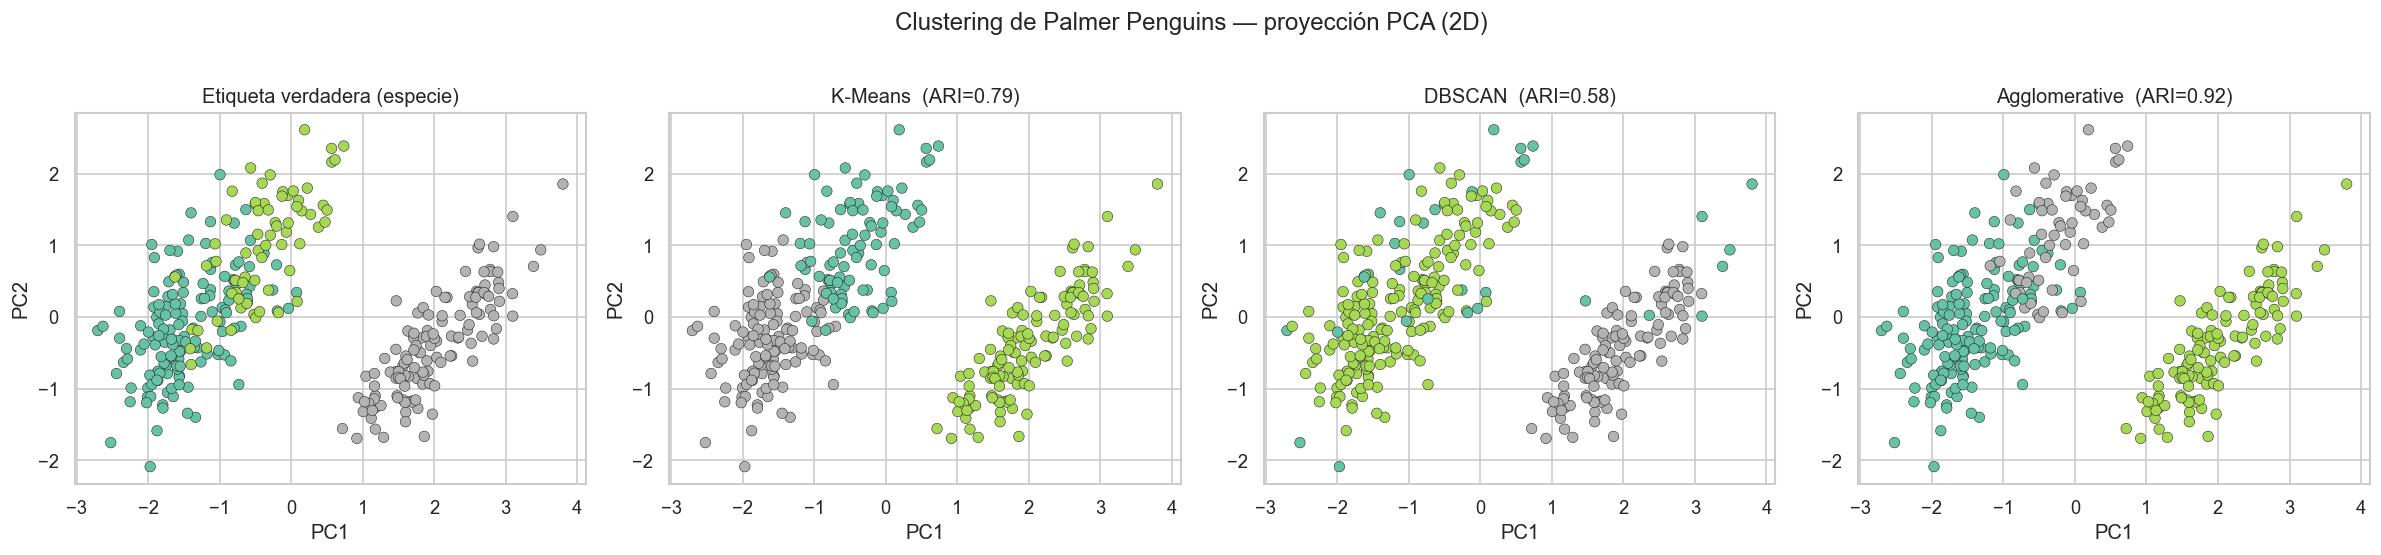
\includegraphics[width=\linewidth]{images/clusters_pca.png}
\caption{Proyección PCA 2D de las 333 observaciones. De izquierda a derecha: etiqueta verdadera de especie, K-Means, DBSCAN y Agglomerative. El ARI consignado en el título de cada panel corresponde al modelo correspondiente.}
\label{fig:pca}
\end{figure}

\subsection{Matriz de confusión del mejor modelo}

Dado que Agglomerative obtiene el mayor ARI, se reporta su matriz de confusión contra la verdad de campo. La figura~\ref{fig:confmat} muestra que los clusters numéricos asignados por el algoritmo se corresponden con las tres especies con un error de asignación pequeño concentrado en la frontera \emph{Adelie}/\emph{Chinstrap}.

\begin{figure}[H]
\centering
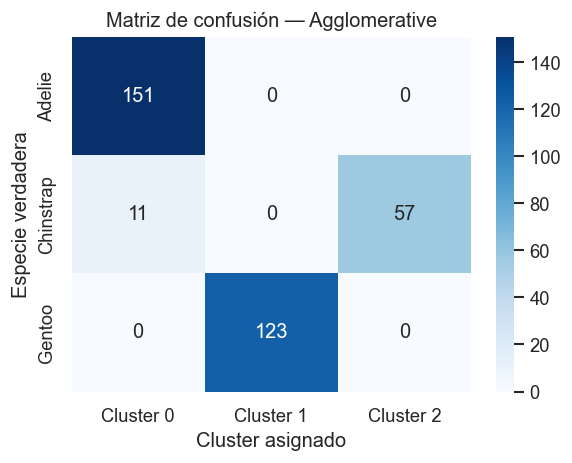
\includegraphics[width=0.6\linewidth]{images/confusion.png}
\caption{Matriz de confusión de Agglomerative Clustering (linkage=Ward) contra la etiqueta verdadera de especie. El emparejamiento cluster--especie es directo y reproduce la estructura biológica.}
\label{fig:confmat}
\end{figure}

\subsection{Discusión}

Los resultados confirman parcialmente la hipótesis. \textbf{Agglomerative} con linkage de Ward es el algoritmo más preciso en términos de ARI (0.916), seguido por \textbf{K-Means} (0.793). Ambos métodos asumen clusters convexos de varianza similar --- supuesto que se cumple razonablemente en este dataset tras estandarización.

\textbf{DBSCAN} obtiene la mejor compacidad interna (Silhouette $=0.557$) porque ignora los 33 puntos marcados como ruido, lo que infla artificialmente la métrica. En la práctica, fusiona \emph{Adelie} y \emph{Chinstrap} en un único cluster denso, hecho que penaliza su ARI. Una búsqueda fina del par $(\varepsilon, \text{minPts})$ mediante la curva $k$-distance \citep{ester1996density,schubert2017dbscan} podría mejorar su desempeño, pero está fuera del alcance de este trabajo corto.

El comportamiento es congruente con la literatura: para datasets pequeños, de baja dimensionalidad y con clusters geométricamente bien separados, los algoritmos centroide-céntricos y jerárquicos suelen superar a los basados en densidad \citep{xu2005survey,saxena2017review}.
